% SAE-gate internals: encode -> mask selected features -> decode -> delta add
\documentclass[tikz,border=5pt]{standalone}
\usepackage{xcolor}
\usepackage{fontspec}
\usetikzlibrary{arrows.meta,shapes.geometric,calc,shadows.blur,positioning}

% Define color scheme
\definecolor{primaryblue}{RGB}{41,128,185}
\definecolor{secondarygreen}{RGB}{39,174,96}
\definecolor{accentorange}{RGB}{230,126,34}
\definecolor{warningred}{RGB}{231,76,60}
\definecolor{lightgray}{RGB}{236,240,241}
\definecolor{darkgray}{RGB}{52,73,94}

\begin{document}
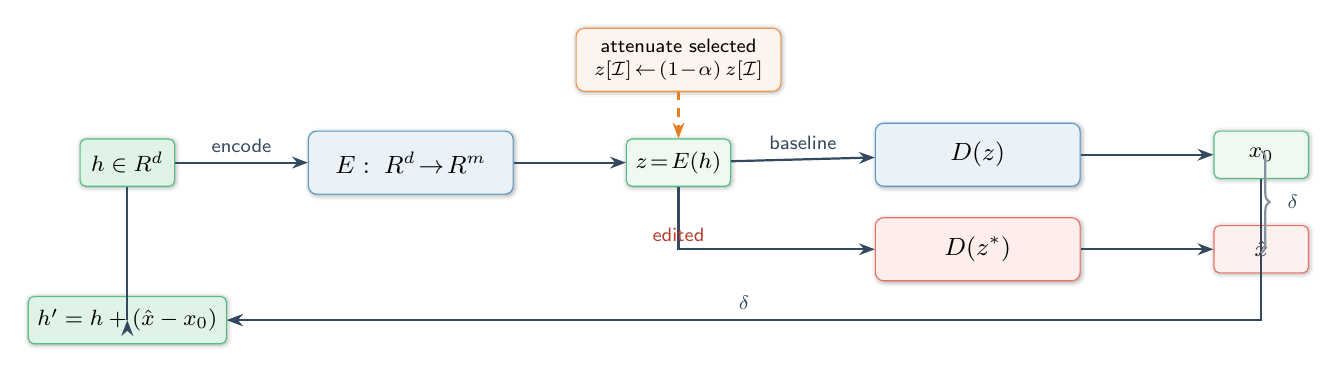
\begin{tikzpicture}[
  node distance=10mm and 14mm,
  block/.style={
    draw=primaryblue!80,
    fill=primaryblue!10,
    rounded corners=3pt,
    minimum width=26mm,
    minimum height=8mm,
    align=center,
    font=\sffamily\small,
    blur shadow={shadow blur steps=5, shadow xshift=0.5pt, shadow yshift=-0.5pt}
  },
  vec/.style={
    draw=secondarygreen!80,
    fill=secondarygreen!8,
    rectangle,
    rounded corners=2pt,
    minimum width=12mm,
    minimum height=6mm,
    align=center,
    font=\sffamily\footnotesize,
    blur shadow={shadow blur steps=3, shadow xshift=0.3pt, shadow yshift=-0.3pt}
  },
  operation/.style={
    draw=accentorange!80,
    fill=accentorange!8,
    rounded corners=3pt,
    minimum width=26mm,
    minimum height=8mm,
    align=center,
    font=\sffamily\scriptsize,
    blur shadow={shadow blur steps=3, shadow xshift=0.3pt, shadow yshift=-0.3pt}
  },
  line/.style={-{Stealth[length=2mm]}, thick, draw=darkgray},
  dashedline/.style={-{Stealth[length=2mm]}, thick, draw=accentorange, dashed}
]

% Hidden state
\node[vec, fill=secondarygreen!15] (h) at (0,0) {$h \in \mathbb{R}^{d}$};

% Encoder
\node[block] (E) at (3.6,0) {$E:\;\mathbb{R}^{d}\!\to\!\mathbb{R}^{m}$};
\draw[line] (h) -- (E) node[midway, above, font=\sffamily\scriptsize, text=darkgray] {encode};

% Latents and mask
\node[vec] (z) at (7.0,0) {$z\!=\!E(h)$};
\node[operation] (mask) at ($(z.north)+(0,10mm)$) {attenuate selected\\$z[\mathcal{I}]\!\leftarrow\! (1\!-\!\alpha)\,z[\mathcal{I}]$};
\draw[dashedline] (mask) -- (z);
\draw[line] (E) -- (z);

% Decoder baseline and edited
\node[block] (D0) at (10.8,1.0mm) {$D(z)$};
\node[block, fill=warningred!10, draw=warningred!80] (D1) at (10.8,-11mm) {$D(z^{\ast})$};
\draw[line] (z) -- (D0) node[midway, above, font=\sffamily\scriptsize, text=darkgray] {baseline};
\draw[line] (z) |- (D1) node[near start, below, font=\sffamily\scriptsize, text=warningred!80!black] {edited};

% Delta and apply
\node[vec] (x0) at (14.4,1.0mm) {$x_0$};
\node[vec, fill=warningred!8, draw=warningred!80] (x1) at (14.4,-11mm) {$\hat{x}$};
\draw[line] (D0) -- (x0);
\draw[line] (D1) -- (x1);

% Output
\node[vec, fill=secondarygreen!15, minimum width=22mm] (hout) at (0,-20mm) {$h' = h + (\hat{x}-x_0)$};
\draw[line] (h) |- (hout);
\draw[line] (x0) |- (hout) node[near end, above, font=\sffamily\scriptsize, text=darkgray] {$\delta$};
\draw[line] (x1) |- (hout);

% Add brace to show delta computation
\draw[decorate, decoration={brace, amplitude=3pt, mirror}, thick, draw=darkgray!60]
  (14.4,-11.5mm) -- (14.4,1.5mm) node[midway, right=2mm, font=\sffamily\scriptsize, text=darkgray] {$\delta$};

\end{tikzpicture}
\end{document}
